\documentclass{article}
\usepackage{amsmath} % for advanced math environments
\usepackage{amsfonts} % for math fonts
\usepackage{amssymb} % for math symbols
\usepackage{amsthm} % for theorems and proofs
\usepackage{mathtools} % for mathematical tools
\usepackage{mathrsfs} % for script-like fonts in math
\usepackage{bm} % for bold math symbols
\usepackage{bbm} % for "blackboard-style" characters in math
\usepackage{graphicx} % for including graphics
\usepackage{hyperref} % for including hyperlinks
\usepackage{tcolorbox}
\usepackage{tikz}
\tcbuselibrary{theorems, breakable}
\usepackage{xcolor}
\usepackage[margin=1in]{geometry}

\newcommand{\C}{\mathbb{C}}
\newcommand{\N}{\mathbb{N}}
\newcommand{\Q}{\mathbb{Q}}
\newcommand{\R}{\mathbb{R}}
\newcommand{\Z}{\mathbb{Z}}
\newcommand{\pset}{\mathscr{P}}
\DeclareMathOperator{\lcm}{lcm}

% Define a shortcut for \begin{bmatrix} and \end{bmatrix}
\newcommand{\bmat}[1]{\begin{bmatrix}#1\end{bmatrix}}
\newcommand{\cmat}[1]{\begin{pmatrix}#1\end{pmatrix}}

\newtcolorbox[auto counter]{problem}%
{
    breakable,
    colback=cyan!5,
    colframe=cyan!35!black,
    fonttitle=\bfseries,
    title=Problem~\thetcbcounter,
}

\newtcolorbox{solution}[1]
{
    breakable,
    colback=red!5,
    colframe=red!75!black,
    fonttitle=\bfseries,
    title=Solution: #1,
}

% Title
\title{9 Disproof}
\author{Benjamin Basseri}


\begin{document}

\maketitle

Each of the following statements is either true or false. If a statement is true, prove it. If a statement is false, disprove it.

\begin{problem}
If $x, y \in \R$, then $|x + y| = |x| + |y|$.
\end{problem}

\textbf{Solution: show a counterexample.}

The statement is false. Let $x = 1$ and $y = -1$. Then $|x + y| = 0$ but $|x| + |y| = 1 + 1 = 2$.

\begin{problem}
For every natural number $n$, the integer $2n^2 - 4n + 31$ is prime.
\end{problem}

\textbf{Solution: show a counterexample.}

Notice that if $n$ is a multiple of 31 then the polynomial overall just adds different multiples of 31, which will not necessarily be prime. For example when $n = 31$ we have
$$2(31)(31) - 4(31) + (31) = 59(31)$$
which is not prime.

\begin{problem}
If $n \in \Z$ and $n^5 - n$ is even, then $n$ is even.
\end{problem}

\textbf{Solution: applying parity rules, show a counterexample.}
\\
It's possible for $n^5 - n$ to be even when $n$ is odd, since $n^5$ is odd when $n$ is odd, and the difference of two odds is even. Take $n = 1$, then $n^5 - n = 0$ which is even.

\begin{problem}
For every natural number $n$, the integer $n^2 + 17n + 17$ is prime.
\end{problem}

\textbf{Solution: show a counterexample by plugging in multiples of 17}

If $n = 17$, then $n^2 + 17n + 17 = 17(17) + 17(17) + 17 = 17(17 + 17 + 1) = 35(17)$ which is not prime.

\begin{problem}
If $A, B, C$ and $D$ are sets, then $(A \times B) \cup (C \times D) = (A \cup C) \times (B \cup D)$.
\end{problem}

\textbf{Solution: show a counterexample.}
\\
Notice that $(A \times B) \cup (C \times D)$ (the LHS) contains ordered pairs from $A \times B$ or $C \times D$ but not necessarily any members from $C \times B$ or $A \times D$ (the RHS). We can construct a counterexample where $A = \{a\}, B = \{b\}, C = \{c\}, D = \{d\}$. Then $(A \times B) \cup (C \times D) = \{(a, b), (c, d)\}$ but $(A \cup C) \times (B \cup D) = \{(a, b), (a, d), (c, b), (c, d)\}$.

\begin{problem}
If $A, B, C$ and $D$ are sets, then $(A \times B) \cap (C \times D) = (A \cap C) \times (B \cap D)$.
\end{problem}

\textbf{Solution: prove directly.}

Both sets contain pairs whose first coordinate is in both $A$ and $C$ and whose second coordinate is in both $B$ and $D$. The statement is true and we can prove directly:

\begin{align*}
  (A \times B) \cap (C \times d) & = \{(x, y): (x, y) \in A \times B \land (x, y) \in C \times D\} \\
                                 & = \{(x, y): x \in A \land x \in C \land y \in B \land y \in D\} \\
                                 & = (A \cap C) \times (B \cap D).
\end{align*}

\begin{problem}
If $A, B$ and $C$ are sets, and $A \times C = B \times C$, then $A = B$.
\end{problem}

\textbf{Solution: prove contrapositively.}

Suppose $A \neq B$. Then assume WLOG there exists an $a \in A$ but $a \not\in B$. In that case $(a, c) \in A \times C$ but not in $B \times C$, so $A \times C \neq B \times C$ (unless these sets are empty).

\begin{problem}
If $A, B$ and $C$ are sets, then $A - (B \cup C) = (A - B) \cup (A - C)$.
\end{problem}

\textbf{Solution:}
\\
The set $A - (B\cup C)$ contains all $A$ members that do not appear in either $B$ or $C$. However, if $B$ has a member $b$ which is also in $A$ but not in $C$, then $A - B$ removes that member and $A - C$ does not. Then the union would contain that $b$.

\begin{problem}
If $A$ and $B$ are sets, the $\mathscr{P}(A) - \mathscr{P}(B) \subseteq \mathscr{P}(A - B)$.
\end{problem}

\textbf{Solution: disprove with a counterexample.}

Often, disproofs rely on a relation between the objects in question. Suppose $A = \Z$ and $B = 2\Z$ (the even integers). Then $\mathscr{P}(A)$ are all possible subsets of integers while $\mathscr{P}(B)$ are all sets of even integers. Therefore $\mathscr{P}(A) - \mathscr{P}(B)$ will contain sets with both even and odd integers, such as $\{1, 2\}$. However if we remove the even integers from $\Z$ before taking the power set, then we only have odd members to form subsets. Since $2 \not\in A - B$, the set $\{1, 2\}$ is not in $\mathscr{P}(A - B)$.

\begin{problem}
If $A$ and $B$ are sets and $A \cap B = \varnothing$, then $\pset(A) - \pset(B) \subseteq \pset(A - B)$.
\end{problem}
\textbf{Solution: prove directly.}
\\
Given $A$ and $B$ have no members in common we can say that $A - B = A$, so $\pset(A - B) = \pset(A)$, all subsets of $A$. Then $\pset(A) - \pset(B)$ must be contained in $\pset(A)$ since it can only be smaller (in fact the LHS only lacks the empty set, the only set in common between the two power sets).

\begin{problem}
If $a, b \in \N$, then $a + b < ab$.
\end{problem}

\textbf{Solution: show a counterexample.}
\\
If $a = b = 2$ then $a + b = ab = 4$.

\begin{problem}
If $a, b \in \N$ and $ab, bc$ and $ac$ all have the same parity, then $a, b$ and $c$ all have the same parity.
\end{problem}

\textbf{Solution: show a counterexample}

For a product $xy$ to be even either $x$ or $y$ can be even; in a sense the even property acts like a `dominant gene'. Then we can make a counterexample where $a = 1, b = 2, c = 2$. Then $ab, bc, ac$ are all even but $a$ is odd.

\begin{problem}
There exists a set $X$ for which $\R \subseteq X$ and $\varnothing \in X$.
\end{problem}

\textbf{Solution: prove directly with set axioms.}

We can always union any sets together, so $X = \R \cup \{\varnothing\}$ suffices.

\begin{problem}
If $A$, and $B$ are sets, then $\pset(A) \cap \pset(B) = \pset(A \cap B)$.
\end{problem}

\textbf{Solution: prove by mutual inclusion.}
\\
For $X \in \pset(A) \cap \pset(B)$, $X \subseteq A$ and $X \subseteq B$, meaning all $X$ members belong to both $A$ and $B$. Then all those members will be in $A \cap B$ and form a subset in $\pset(A \cap B)$. Conversely, if $X \in \pset(A \cap B)$ then $X$ members must belong to both $A$ and $B$. Since they belong to $A$, $X \in \pset(A)$ and since they belong to $B$, $X \in \pset(B)$. Therefore $X \in \pset(A) \cap \pset(B)$.

\begin{problem}
Every odd integer is the sum of three odd integers
\end{problem}

\textbf{Solution: prove algebraically.}

Since 1 and -1 are odd, we can write any odd integer $2k + 1$ as $(2k + 1) + 1 - 1 = 2k + 1$.

\begin{problem}
If $A$ and $B$ are finite sets, then $|A \cup B| = |A| + |B|$.
\end{problem}
\textbf{Solution: disprove by counterexample.}
\\

We know the statement is false from the Inclusion-Exclusion principle. This equality breaks when $A$ and $B$ have a member in common. For example $A = \{a\} = B$, then $|A \cup B| = 1$ but $|A| + |B| = 2$.

\begin{problem}
For all sets $A$ and $B$, if $A - B = \varnothing$, then $B \neq \varnothing$.
\end{problem}

\textbf{Solution: disprove By counterexample.}
\\

This statement might be true for nonempty sets but as stated, $A$ could be the empty set which would allow $B$ to be anything and $A - B$ would still be empty.

\begin{problem}
If $a, b, c \in \N$, then at least one of $a - b, a + c$ and $b - c$ is even.
\end{problem}

\textbf{Solution: prove by contradiction.}
\\

Suppose all three sums are odd. Then $a - b + a + c + b - c = 2a$ which is even, but this contradicts the fact that the sum of three odds should be odd.

\begin{problem}
For every $r, s \in\Q$ with $r < s$, there exists an irrational number $u$ such that $r < u < s$.
\end{problem}

\textbf{Solution: use direct proof and construct the irrational number.}
\\

The statement seems true, the challenge will be to find $u$ for any $r$ and $s$. The answer will likely be a function of $r$ and $s$ so it can apply to any rational numbers. Also, we know that $\sqrt{2}$ is irrational and any rational multiple $\sqrt{2}\frac{a}{b}$ is still irrational.
\\

Start with $0 < \sqrt{2} < 2$:
\begin{align*}
   & 0 < \sqrt{2} < 2                  &                          \\
   & 0 < \sqrt{2}(s-r) < 2(s-r)        & \text{multiply by $s-r$} \\
   & 0 < \sqrt{2}\frac{s-r}{2} < s-r   & \text{divide by 2}       \\
   & r < r + \sqrt{2}\frac{s-r}{2} < s & \text{add $r$}
\end{align*}

\begin{problem}
There exist prime numbers $p$ and $q$ for which $p - q = 1000$.
\end{problem}

\textbf{Solution: find an example.}
\\

On the surface there's little reason to doubt the statement, that two primes could differ by 1000. Using a computer program or looking up a list of primes, we can find that 1013 and 13 are both primes, and their difference is 1000.

\begin{problem}
There exist prime numbers $p$ and $q$ for which $p - q = 97$
\end{problem}

\textbf{Solution: disprove using arithmetic properties of primes.}
\\

This claims there are two primes that differ by 97, an odd number. Except for 2, all primes are odd so the difference between them is even. This means that $q$ must equal 2 in order to have an odd difference with another prime. However, 99 is not prime, so the statement is false.

\begin{problem}
If $p$ and $q$ are prime numbers for which $p < q$, then $2p + q^2$ is odd.
\end{problem}

\textbf{Solution: prove directly using parity properties}
\\

In the sum $2p + q^2$, the term $2p$ is even. The only way for $q^2$ to be even is if $q = 2$, the only even prime. However we're given $q$ is strictly greater than prime $p$, so $q$ is a prime at least 3 and therefore odd. This makes $q^2$ odd as well, so the sum is an even plus an odd, which is odd.

\begin{problem}
If $x, y \in \R$ and $x^3 < y^3$, then $x < y$.
\end{problem}

\textbf{Solution: prove directly}
\\

Cubing is an order-preserving operation so this is true. Given $x^3 < y^3$, assume $y > 0$. Then we have:
\begin{align*}
  x^3                       & < y^3 \\
  \frac{x^3}{y^3}           & < 1   \\
  \sqrt[3]{\frac{x^3}{y^3}} & < 1   \\
  \frac{x}{y}               & < 1   \\
\end{align*}

Similar reasoning works for $y = 0$ and $y < 0$.

\begin{problem}
The inequality $2^x \geq x + 1$ is true for all positive real numbers $x$.
\end{problem}

\textbf{Solution: graph and inspect}
\\

By plotting $2^x$ and $x + 1$ we can see there is a region around 1/3 where $x + 1$ exceeds $2^x$. Indeed, plugging in $x = 1/2$ we get $2^x = \sqrt{2} \approx 1.41$ which is less than $1/2 + 1 = 1.5$.

\begin{problem}
For all $a, b, c \in \Z$, if $a \mid bc$, then $a \mid b$ or $a \mid c$.\
\end{problem}

\textbf{Solution: disprove with a counterexample.}
\\

The statement is false since $bc$ could be combining distinct factors from $b$ and $c$ that make it divisible by $a$. For instance suppose $b = 2$ and $c = 3$. Then set $a = 6$ and $a \mid bc$ but $a$ cannot divide $b$ or $c$ alone.

\begin{problem}
Suppose $A, B$ and $C$ are sets. If $A = B - C$, then $B = A \cup C$.
\end{problem}

\textbf{Solution: disprove with a counterexample.}
\\

Sketching a venn diagram hints this is not true:


\begin{center}
  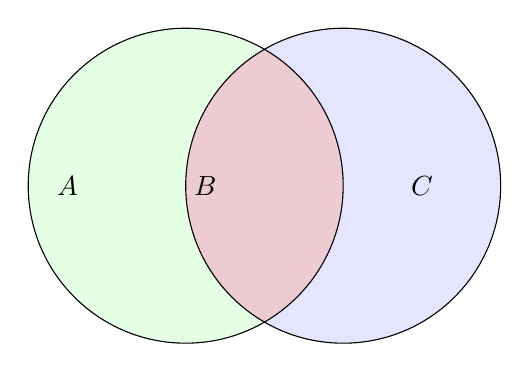
\begin{tikzpicture}
    \fill[green!20, opacity=0.5] (0,0) circle (2cm);
    \fill[blue!20, opacity=0.5] (2,0) circle (2cm);
    \begin{scope} % Scope for 'clip' and 'fill'
      \clip (0,0) circle (2cm);
      \fill[red!30, opacity=0.5] (2,0) circle (2cm);
    \end{scope}
    \draw (0,0) circle (2cm);
    \draw (2,0) circle (2cm);
    \node at (-1.5,0) {$A$}; % Move the A label to the left
    \node at (0.25, 0) {$B$};
    \node at (3, 0) {$C$};
  \end{tikzpicture}
\end{center}

If $C$ contains elements not in $B$ then $A \cup C$ will have these elements but $B$ will not, so $B \neq A \cup C$.

\begin{problem}
The equation $x^2 = 2^x$ has three real solutions.
\end{problem}

By graphing the two functions we see they intersect at the points: 2, 4, and something between -0.5 and -1. Indeed, plugging in $x = -0.5$ makes $x^2 - 2^x < 0$ while $x = -1$ makes $x^2 - 2^x > 0$. By the intermediate value theorem, this tells us there must be another solution in that interval.

\begin{problem}
Suppose $a, b \in \Z$. If $a \mid b$ and $b \mid a$, then $a = b$.
\end{problem}

\textbf{Solution: prove directly.}
\\

Think of the prime decompositions $p_1^{a_1}p_2^{a_2}\ldots$ for $a$ and $p_1^{b_1}p_2^{b_2}\ldots$ for $b$. For $a$ to divide $b$ it must be that the exponent on each prime is less than or equal to each of $b$'s exponents: $a_i \leq b_i, \forall i$. But since $b$ divides $a$ the same is true in reverse: $b_i \leq a_i, \forall i$. This means $a_i = b_i, \forall i$ which means $a$ and $b$ have the same prime factorization, making them equal.

\begin{problem}
If $x, y \in \R$ and $|x + y| = |x - y|$, then $y = 0$.
\end{problem}

\textbf{Solution: disprove with a counterexample.}
\\

All that $|x + y| = |x -y|$ says is that $x$ is the same distance from $y$ as it is from $-y$. If $x = 0$ this is true of any $y$.

\begin{problem}
There exist integers $a$ and $b$ for which $42a + 7b = 1$.
\end{problem}
\textbf{Solution: disprove by contradiction.}
\\

Suppose there are such integers $a, b$. Then we have
$$42a + 7b = 1 \implies 7(6a) + 7b = 1 \implies 7(6a + b) = 1$$
This implies that 7 divides 1, or that $6a + b = 1/7$, neither of which are possible.

\begin{problem}
No number (other than 1) appears in Pascal's triangle more than four times.
\end{problem}
\textbf{Solution: disprove with a counterexample.}
\\

With a computer program we can look for binomial coefficients that appear at least 5 times. Doing so we find 3003 is one such number, the result of $\binom{14}{6}, \binom{14}{8}, \binom{15}{5}, \binom{15}{10}$, and $\binom{78}{2}$.

\begin{problem}
If $n, k \in \N$ and $\binom{n}{k}$ is a prime number, then $k = 1$ or $k = n - 1$.
\end{problem}

\textbf{Solution: prove with direct proof}

If $k = 1$ then $\binom{n}{k} = \frac{n!}{(n-1)!} = n$, and the same for $k = n - 1$. Then it is quite possible for $n$ to be prime. However, for any other value of $k$ the binomial coefficient becomes $\frac{n(n-1)\ldots(n-k+1)}{k!}$.

\textbf{Solution: prove using contrapositive.}
\\

The contrapositive statement is if $k \neq 1$ and $k \neq n - 2$ then $\binom{n}{k}$ is not prime. Indeed, if $k = 0$ or $n$ then we have $\binom{n}{0} = \binom{n}{n} = 1$ which is not prime. If instead $k$ is between 2 and $n - 2$ inclusive, we need to show $\binom{n}{k}$ is composite. Write out $\binom{n}{k}$:
$$\binom{n}{k} = \frac{n(n-1)\ldots(n-k+1)}{k!} = \frac{n(n-1)\ldots(n-k+1)}{k(k-1)\ldots(2)(1)}$$

Now the denominator is $k$ factors but if we ignore the factor 1, the denominator has $k -1$ factors. The numerator meanwhile has $k$ factors for $k \geq 2$. Since the numerator has at least two factors, which are consecutive integers, it must be even and divisible by 2. In fact for $n > 3$ the numerator will be divisible by 4 so we can cancel out the 2 in the denominator, and it does not affect the number of factors in the numerator (for $n \leq 3$ confirm by inspection). This leaves us with $k - 2$ `active' factors in the denominator and $k$ factors in the numerator. At most, each factor in the denominator can cancel out one factor in the numerator, so the fraction simplifies to an integer with at least two factors, making it composite.

\begin{problem}
Suppose $f(x) = a_0 + a_1x + a_2 x^2 + \ldots + a_n x^n$ is a polynomial of degree 1 or greater, and for which each coefficient $a_i$ is in $\N$. Then there is a $k \in \N$ for which the integer $f(k)$ is not prime.
\end{problem}
\textbf{Solution: use relations within the problem to prove.}
\\

Since all the coefficients are natural, we have $f(1) > 1$. Let $f(1) = b$, then $f(x) - b$ has a root at 1. Factor it out to get $f(x) - b = (x - 1)g(x)$ for some polynomial $g(x)$. Note that $g(x)$ must have integer coefficients since by polynomial long division, dividing $a_n x^n + a_{n-1}x^{n-1} + \ldots + a_0$ by $x - 1$ leaves the coefficients the differences of natural numbers.
\\

Back to $f(x) - b = (x - 1)g(x)$: moving $b$ to the RHS gives $f(x) = (x - 1)g(x) + b$. Now we want to show that we can find a composite for $f(x)$, but it has this $b$ term in it. Plugging in $b$ for $x$ doesn't quite work but when we plug in $b + 1$ we get:
$$f(b + 1) = (b)g(b+1) + b = b(g(b+1) + 1)$$

We already have $b > 1$, if $g(b+1) > 1$ then for sure $f(b + 1)$ is composite. Since $g(x)$ has integer coefficients, $g(b+1)$ must be positive because $b + 1$ is positive. When a polynomial with integer coefficients has a positive

\begin{problem}
If $X \subseteq A \cup B$, then $X \subseteq A$ or $X \subseteq B$.
\end{problem}
\textbf{Solution: prove by showing a counterexample.}
\\

Sketching a Venn diagram hints the statement is false. It's possible $X$ contains elements from $A$ that are not in $B$ and elements from $B$ that are not in $A$. Then it's a subset of the union but not either set indidually. For example let $A = \{1, 2\}$ and $B = \{2, 3\}$, then $X = \{1, 3\}$ is a subset of $A \cup B$ but not of $A$ or $B$.

\begin{problem}
In Chapter 5, Exercise 25 asked you to prove that if $2^n - 1$ is prime, then $n$ is prime. Is the converse true?
\end{problem}
\textbf{Solution: disprove with a counterexample.}
\\

By testing the first few prime numbers we find that when $n = 11$ we have $2^{11} - 1 = 2047 = 23 \times 89$. So it is not generally true that if $n$ is prime you have $2^n - 1$ is prime.

\end{document}